% !TeX encoding = UTF-8

\documentclass{protokol}

\usepackage{tikz}
\usetikzlibrary{calc}
\usetikzlibrary{arrows}

%====== Units =====
\usepackage{siunitx}
\sisetup{inter-unit-product =\ensuremath{\cdot}}
\sisetup{group-digits = integer}
\sisetup{output-decimal-marker = {,}}
\sisetup{exponent-product = \ensuremath{\cdot}}
\sisetup{separate-uncertainty}
\sisetup{tight-spacing = false}
%\sisetup{scientific-notation = true}
%\sisetup{round-mode=places,round-precision=4}
%\sisetup{evaluate-expression}


%====== Grafy =====
\usepackage{pgfplots}
\pgfplotsset{width=0.8\linewidth, compat=1.17}
\def\plotcscale{0.8}
\usepackage{pgfplotstable}
\usepackage[figurename=Graf]{caption} % figure caption rename
%====== Rovnice align block ======
\usepackage{amsmath}
\setlength{\jot}{10pt} % rozestup mezi řádky

\graphicspath{ {./img/} }

%====== Vyplňte údaje ======
\jmeno{Jakub Charvot}
\kod{240844}
\rocnik{2.}
\obor{MET}
\skupina{MET/4}
\spolupracoval{Radek Kučera}

\merenodne{10.\,11.\,2022}
\odevzdanodne{24.\,11.\,2022}
\nazev{Operační usměrňovače}
\cislo{4} %měřené úlohy

\predmet{Analogové elektronické obvody}
\ustav{Ústav mikroelektroniky}
\skola{FEKT VUT v Brně}

\def\para{x+0}
\def\parb{\para-80}

% CSV
\usepackage{blindtext}

\usepackage{subfiles} % Best loaded last in the preamble
\usepackage{datatool}


\DTLloaddb[omitlines=2]{prvni}{data/u-na-deltaT.csv}
\DTLloaddb{casova}{data/casova-zavislost.csv}
\DTLloaddb{frekvence}{data/frekvence.csv}


\begin{document}
	%====== Vygenerování tabulky ======
%	\maketitle
	%====== Úvodní texty protokolu ======

%	\section{Teoretický úvod}
%		\begin{figure}[h!]
    \centering
    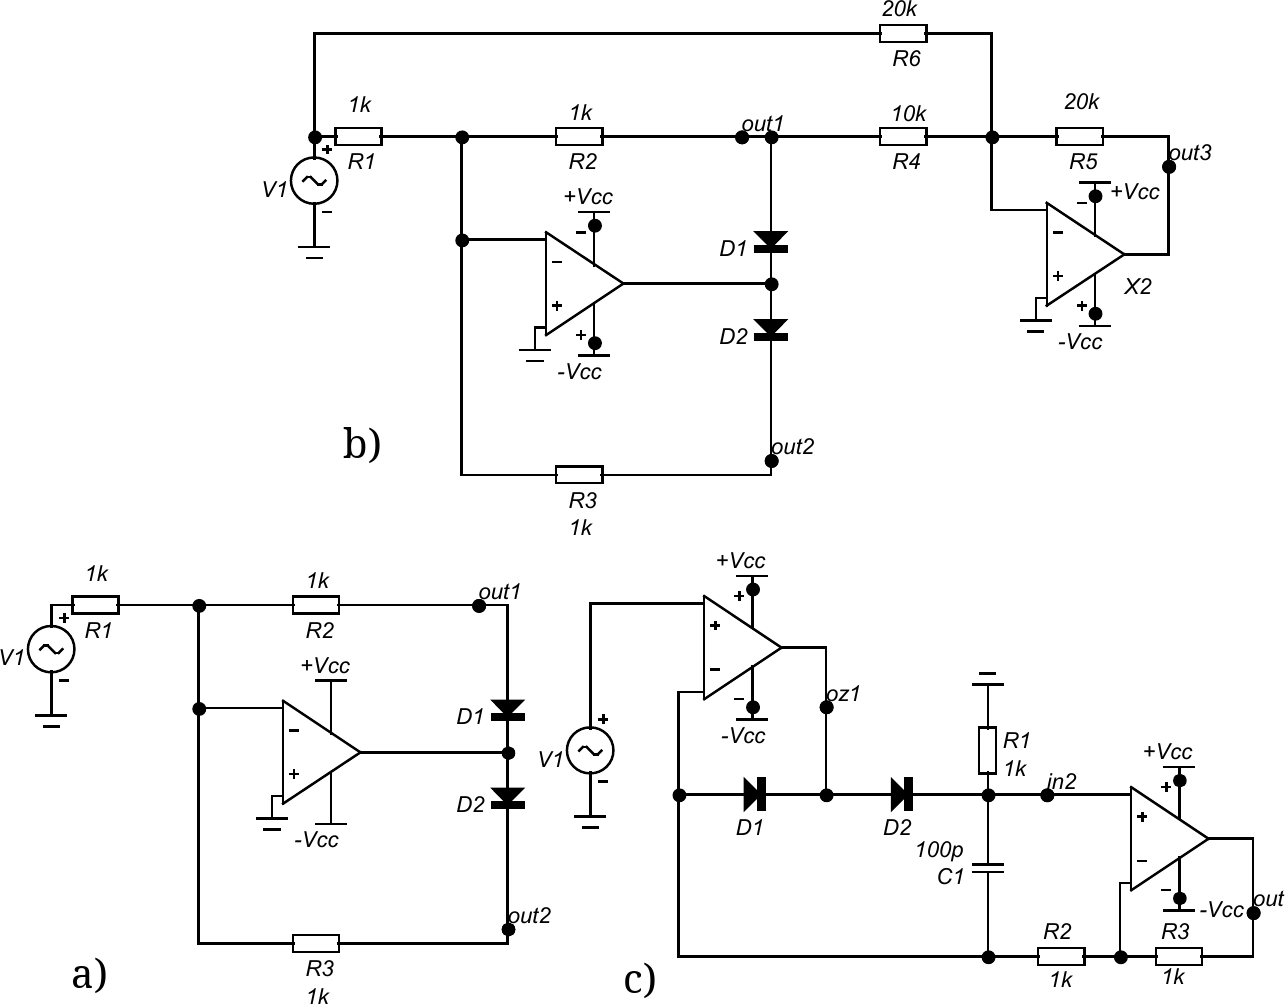
\includegraphics[width=\textwidth]{schema.png}
    \centering
    \caption{Schémata zapojení -- a) jednocestný usměrňovač, b) dvoucestný usměrňovač, c) dvoucestný usměrňovač s minimem přesných součástek.}
    \label{fig:schema}
\end{figure}



\subsection{Funkce jednotlivých zapojení}

    Operační zesilovač s OZ má za úkol překonat nedostatky, které má zapojení pouze s diodami, které díky svému prahovému napětí nedokáží usměrňovat velmi malá napětí. 
    
    Zapojení 1a) je jednocestný usměrňovač, kdy je vždy přes jednu diodu uzavřená záporná zpětná vazba a druhá dioda je uzavřená. Na výstupu je pak signál jednocestně usměrněný a invertovaný. 
    
    Zapojení 1b) pak tento signál zdvojnásobí a sečte s původním vstupním signálem, ve výsledku tedy původní záporné půlvlny zůstanou a kladné po sečtení odpovídají opět záporným. Výsledkem je tedy dvoucestně usměrněný invertovaný signál. 
    Nevýhodou tohoto zapojení je nutnost použít dva co nejshodnější odpory a k nim jeden, který odpovídá hodnotu přesně polovině, při nedodržení nebudou na výstupu půlvlny stejně velké, toto značně zdražuje zapojení. 

    Tento problém se snaží řešit zapojení 1c), kdy pro správnou funkci stačí jedna dvojice přesných odporů \( R_2\) a \(R_3\). Záporná zpětná vazba prvního OZ je vždy uzavřena přes druhý OZ, díky diodám je ale cesta zpětné vazby jiná pro kladný a pro záporný signál, takže ve výsledku je na výstupu druhého OZ signál vždy kladný, neboli dvoucestně usměrněný.   
%		
%	% \newpage
%	\section{Výsledky počítačové simulace}
%		\begin{figure}[h!]
    \centering
    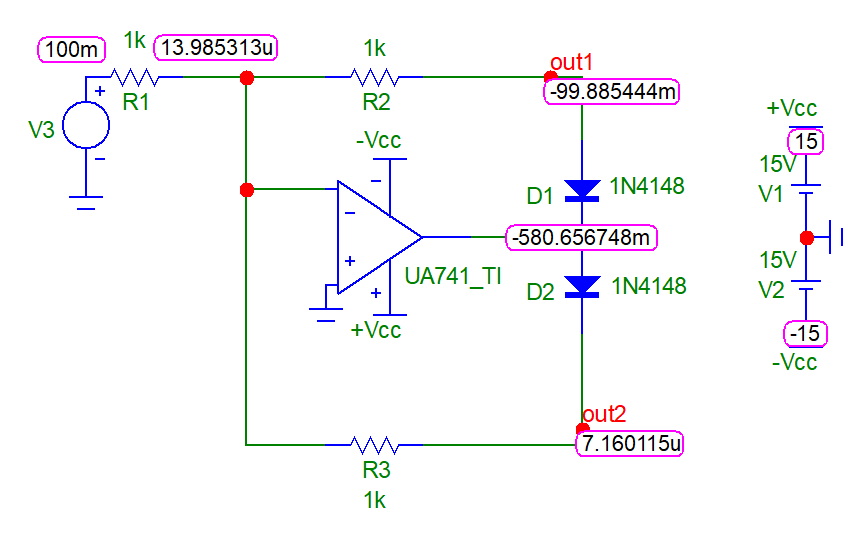
\includegraphics[width=0.63\textwidth]{microcap/1-dcbod.png}
    \caption{Zapojení a) -- stejnosměrný prac. bod pro kladné vstupní napětí.}
    \label{fig:microcap/.png}
\end{figure}

\begin{figure}[h!]
    \centering
    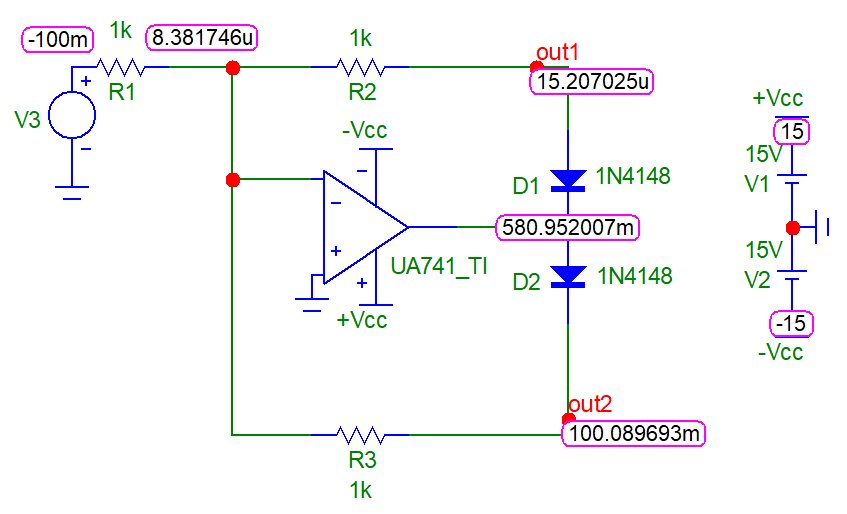
\includegraphics[width=0.63\textwidth]{microcap/1-dcbod2.png}
    \caption{Zapojení a) -- stejnosměrný prac. bod pro záporné vstupní napětí.}
    \label{fig:microcap/.png}
\end{figure}

\begin{figure}[h!]
    \centering
    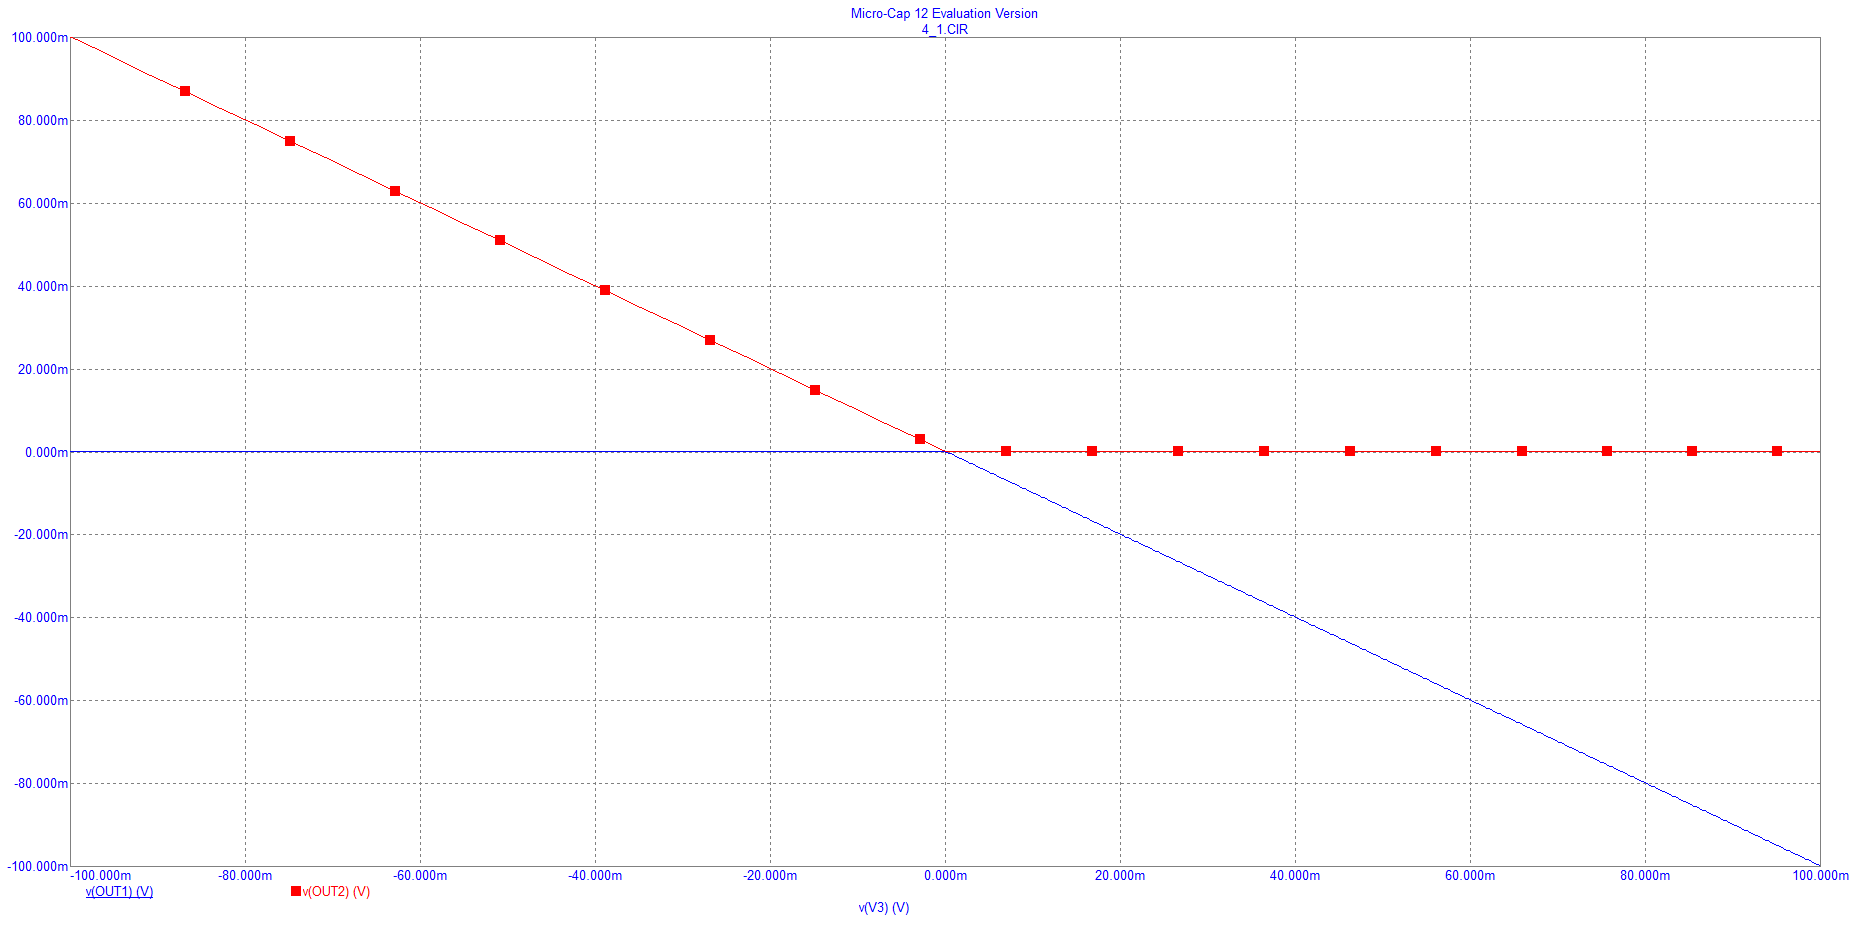
\includegraphics[width=0.8\textwidth]{microcap/1-dcprevodni.png}
    \caption{Zapojení a) -- stejnosměrná převodní charakteristika.}
    \label{fig:microcap/.png}
\end{figure}

\begin{figure}[h!]
    \centering
    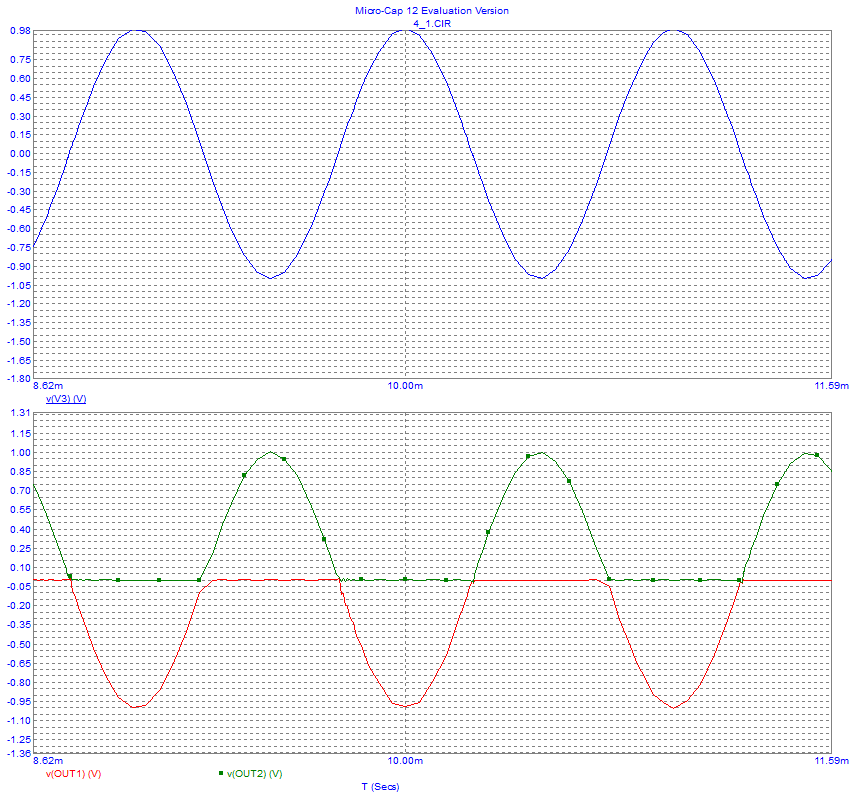
\includegraphics[width=0.8\textwidth]{microcap/1-transient-1khz-1v.png}
    \caption{Zapojení a) -- časová závislost obou výstupních napětí na vstupním napětí, jednocestné zesílení, \(f=\qty{1}{\kilo\hertz}, U_M=\qty{1}{\volt}\).}
    \label{fig:microcap/.png}
\end{figure}

\begin{figure}[h!]
    \centering
    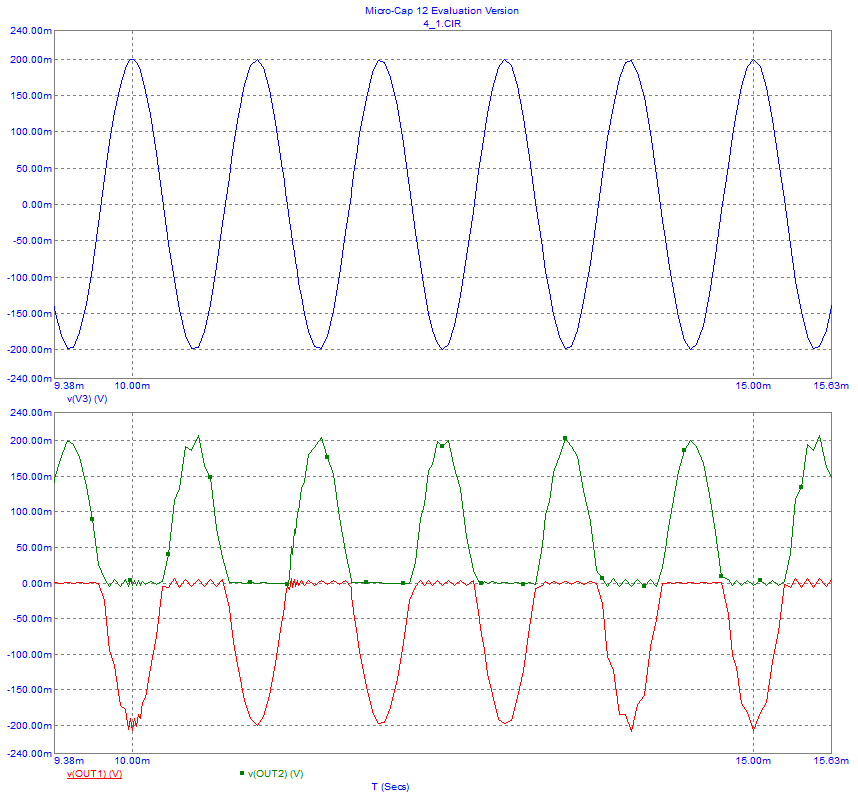
\includegraphics[width=0.7\textwidth]{microcap/1-transient-1khz-0.2v.png}
    \caption{Zapojení a) -- časová závislost obou výstupních napětí na vstupním napětí, nejmenší amplituda, při které zapojení obstojně usměrňuje, \(f=\qty{1}{\kilo\hertz}, U_M=\qty{200}{\milli\volt}\).}
    \label{fig:microcap/.png}
\end{figure}

\begin{figure}[h!]
    \centering
    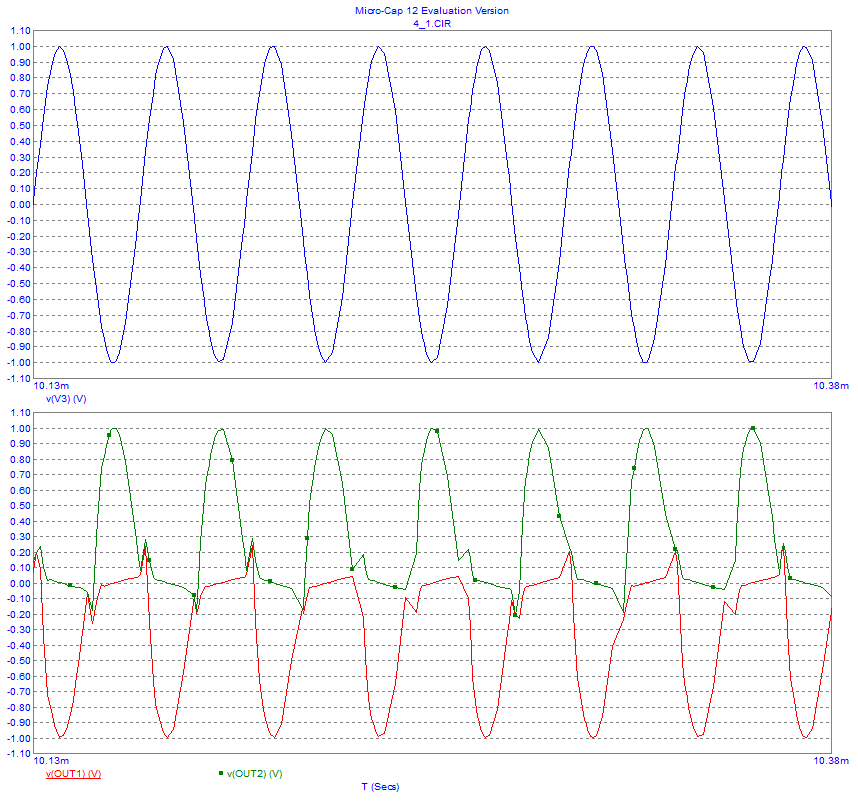
\includegraphics[width=0.7\textwidth]{microcap/1-transient-30khz-1v.png}
    \caption{Zapojení a) -- časová závislost obou výstupních napětí na vstupním napětí, nejvyšší frekvence, při které zapojení obstojně usměrňuje, \(f=\qty{30}{\kilo\hertz}, U_M=\qty{1}{\volt}\).}
    \label{fig:microcap/.png}
\end{figure}

\begin{figure}[h!]
    \centering
    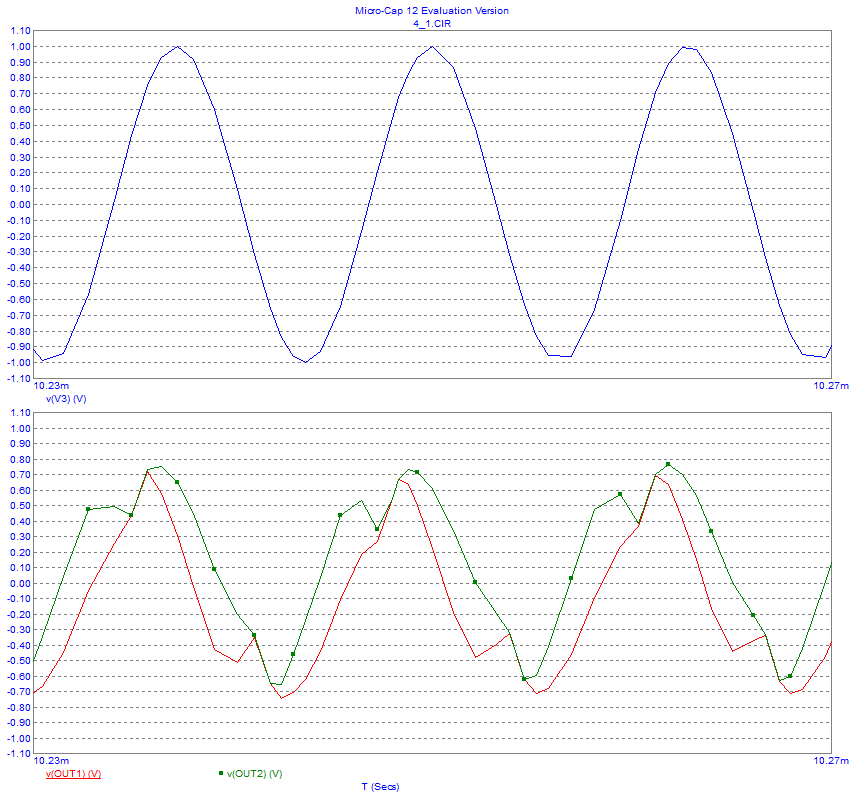
\includegraphics[width=0.8\textwidth]{microcap/1-transient-100khz-1v.png}
    \caption{Zapojení a) -- časová závislost obou výstupních napětí na vstupním napětí, příliš vysoká frekvence, k usměrnění nedochází vůbec, \(f=\qty{100}{\kilo\hertz}, U_M=\qty{1}{\volt}\).}
    \label{fig:microcap/.png}
\end{figure}    

% \begin{figure}[h!]
%     \centering
%     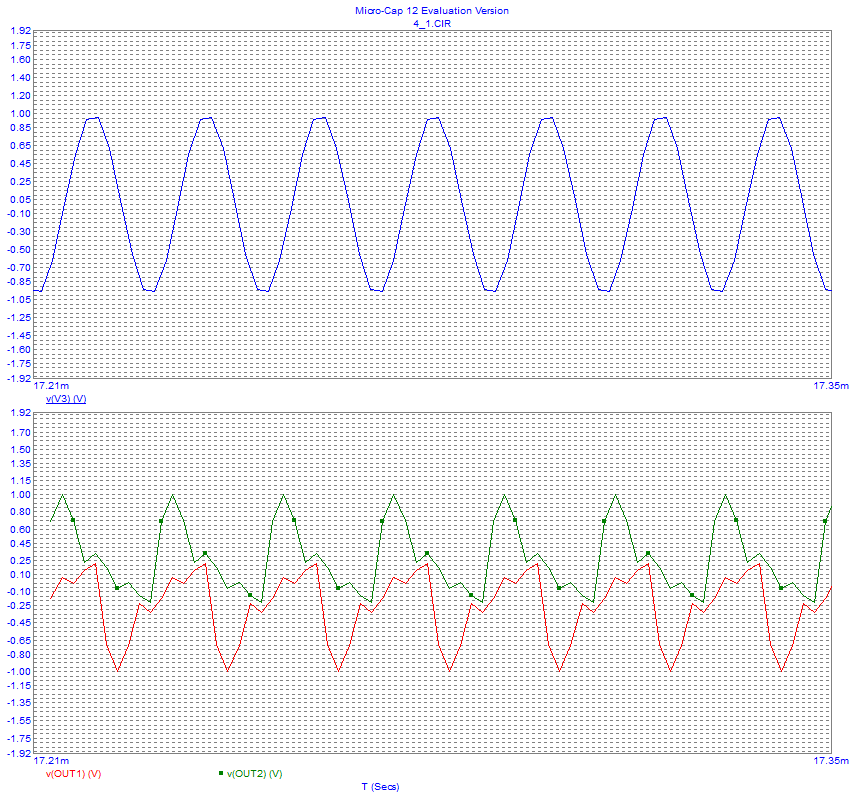
\includegraphics[width=0.8\textwidth]{microcap/1-transient-50khz-1v.png}
%     \caption{microcap/.png}
%     \label{fig:microcap/.png}
% \end{figure}

\begin{figure}[h!]
    \centering
    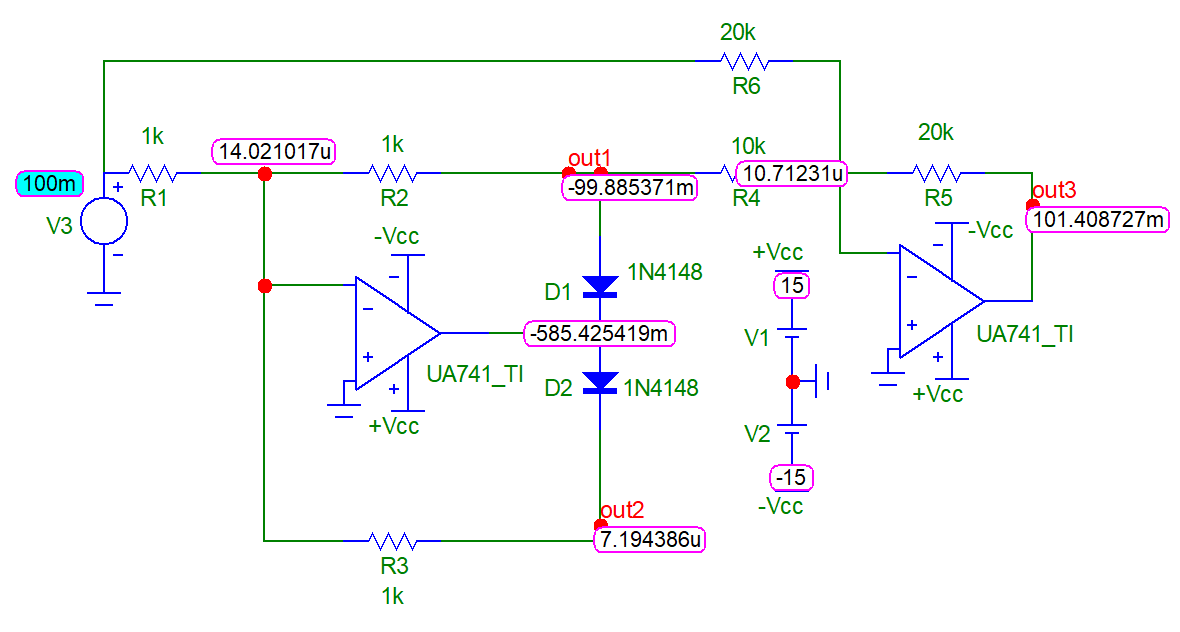
\includegraphics[width=0.8\textwidth]{microcap/2-dcbod.png}
    \caption{Zapojení b) -- stejnosměrný prac. bod při kladném napětí na vstupu, na výstupu kladné napětí.}
    \label{fig:microcap/.png}
\end{figure}

\begin{figure}[h!]
    \centering
    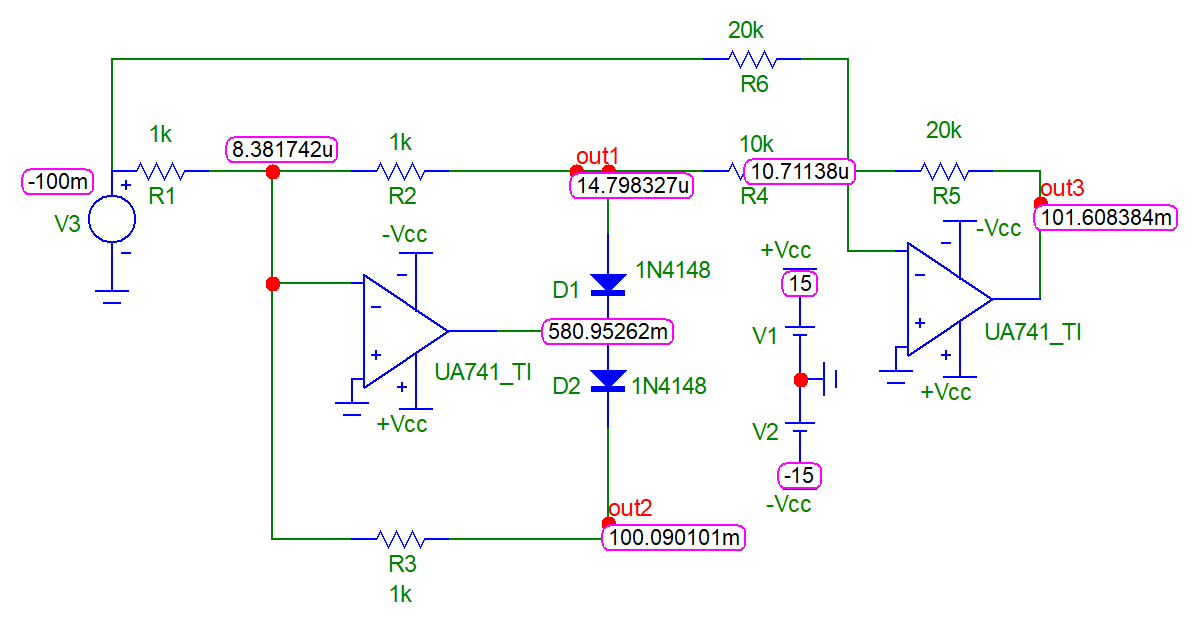
\includegraphics[width=0.61\textwidth]{microcap/2-dcbod2.png}
    \caption{Zapojení b) -- stejnosměrný prac. bod při záporném napětí na vstupu, na výstupu opět kladné napětí.}
    \label{fig:microcap/.png}
\end{figure}

\begin{figure}[h!]
    \centering
    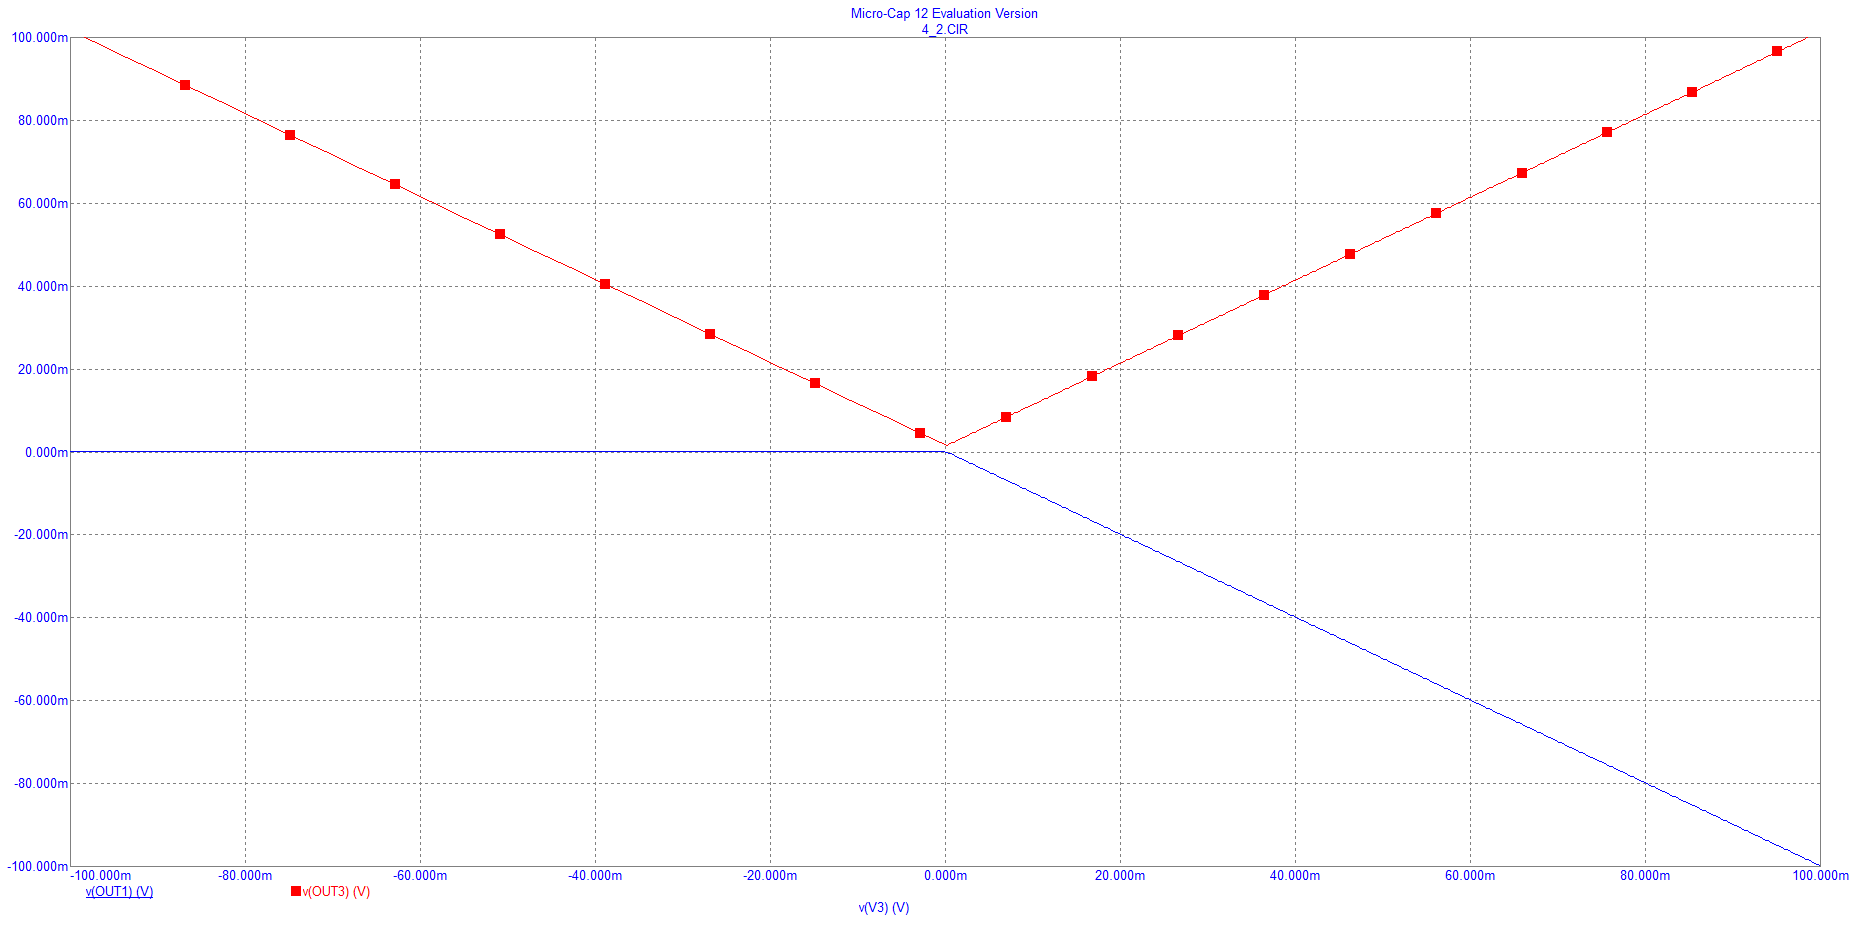
\includegraphics[width=0.61\textwidth]{microcap/2-dcprevodni.png}
    \caption{Zapojení b) -- stejnosměrná převodní charakteristika dvoucestného usměrnění.}
    \label{fig:microcap/.png}
\end{figure}

\begin{figure}[h!]
    \centering
    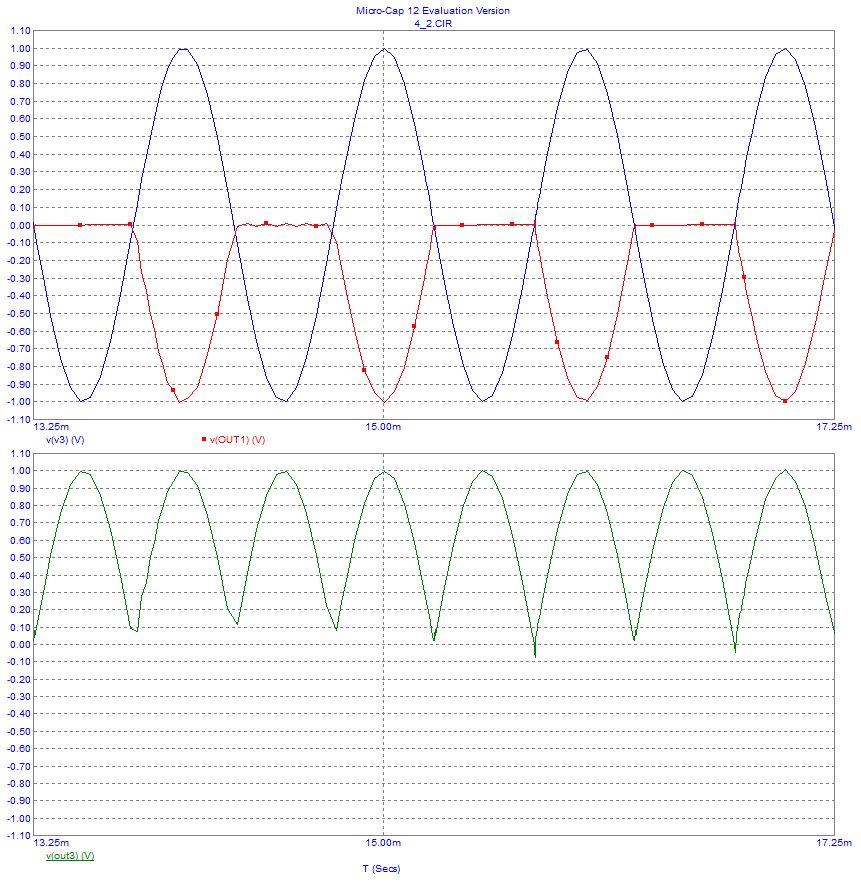
\includegraphics[width=0.61\textwidth]{microcap/2-transient-1khz-1v.png}
    \caption{Zapojení b) -- časová závislost napětí na výstupech obou OZ na vstupním napětí, jednocestné a dvoucestné usměrnění, \(f=\qty{1}{\kilo\hertz}, U_M=\qty{1}{\volt}\).}
    \label{fig:microcap/.png}
\end{figure}

% \begin{figure}[h!]
%     \centering
%     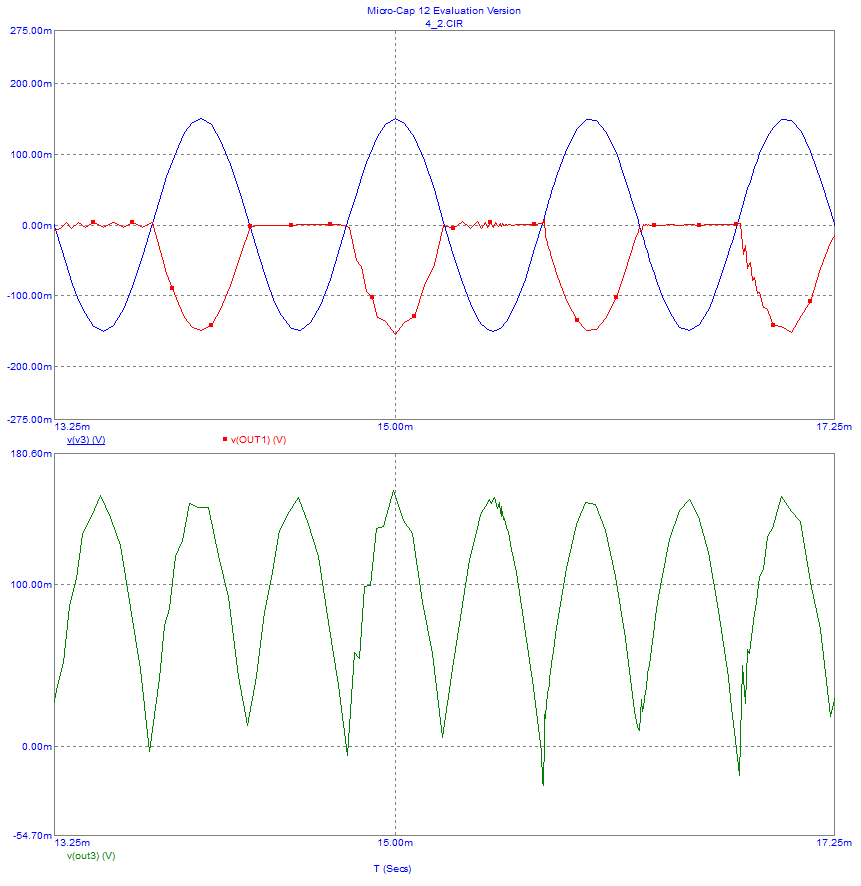
\includegraphics[width=0.8\textwidth]{microcap/2-transient-1khz-0.15v.png}
%     \caption{Zapojení b) -- časová závislost napětí na výstupech obou OZ na vstupním napětí, nejmenší amplituda, při které uspokojivě usměrňuje, \(f=\qty{1}{\kilo\hertz}, U_M=\qty{150}{\milli\volt}\).}
%     \label{fig:microcap/.png}
% \end{figure}

\begin{figure}[h!]
    \centering
    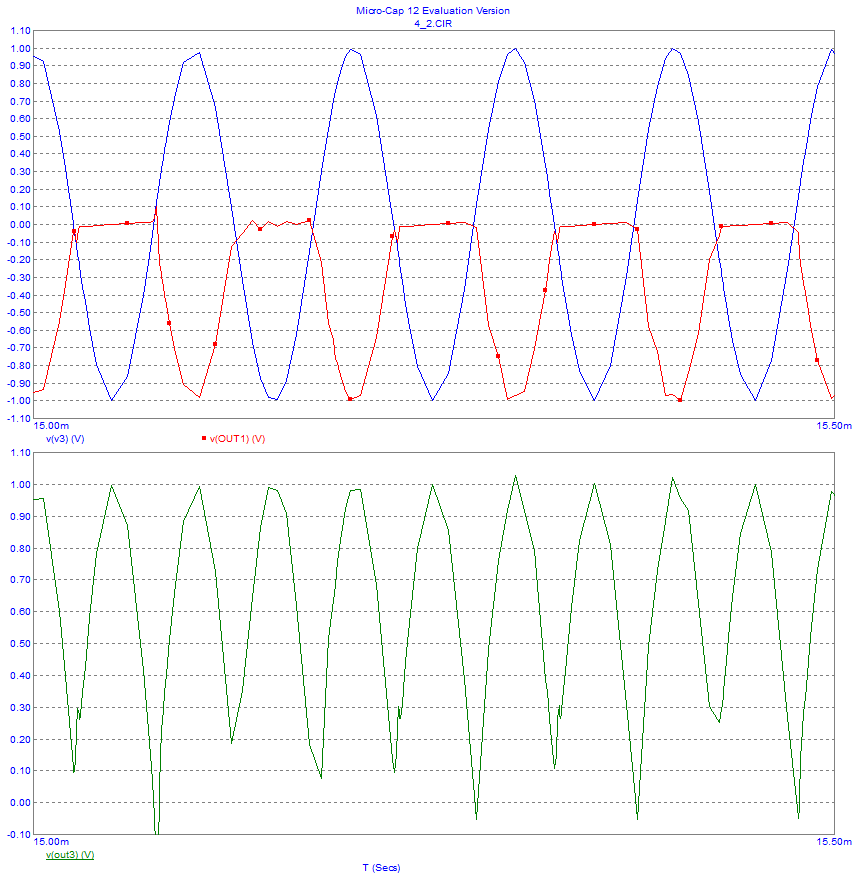
\includegraphics[width=0.7\textwidth]{microcap/2-transient-10khz-1v.png}
    \caption{Zapojení b) -- časová závislost napětí na výstupech obou OZ na vstupním napětí, nejvyšší frekvence, při které uspokojivě usměrňuje, \(f=\qty{10}{\kilo\hertz}, U_M=\qty{1}{\volt}\).}
    \label{fig:microcap/.png}
\end{figure}

\begin{figure}[h!]
    \centering
    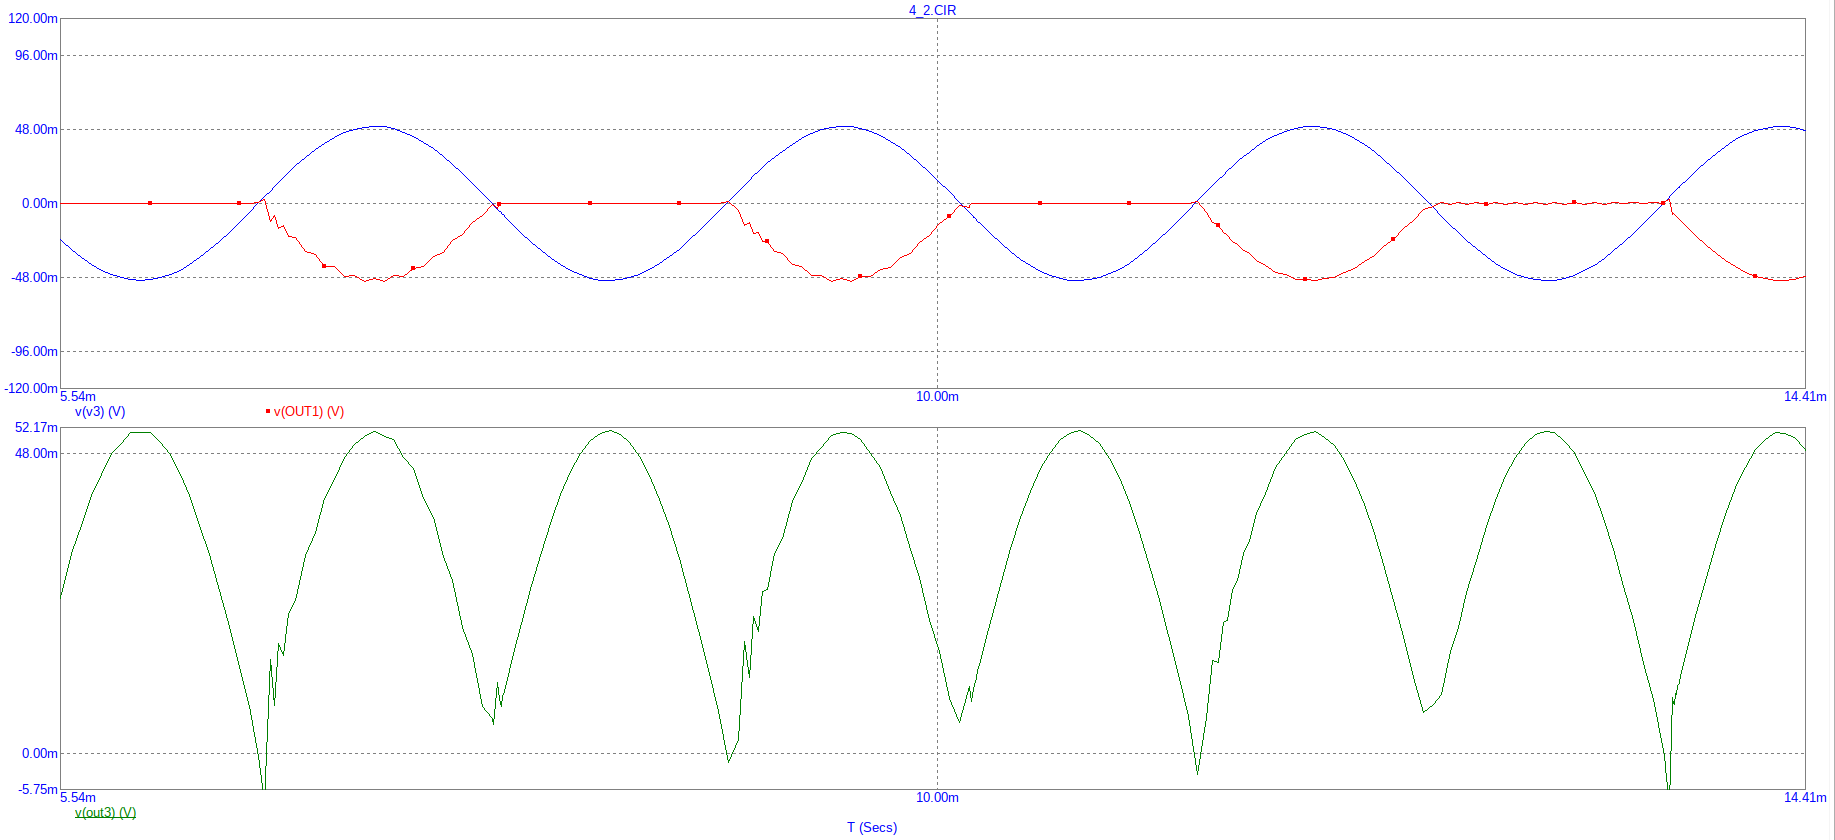
\includegraphics[width=0.7\textwidth]{microcap/2-transient-420hz-0.05v.png}
    \caption{Zapojení b) -- časová závislost napětí na výstupech obou OZ na vstupním napětí, nejnižší amplituda, při které uspokojivě usměrňuje, \(f=\qty{420}{\hertz}, U_M=\qty{50}{\milli\volt}\).}
    \label{fig:microcap/.png}
\end{figure}

\begin{figure}[h!]
    \centering
    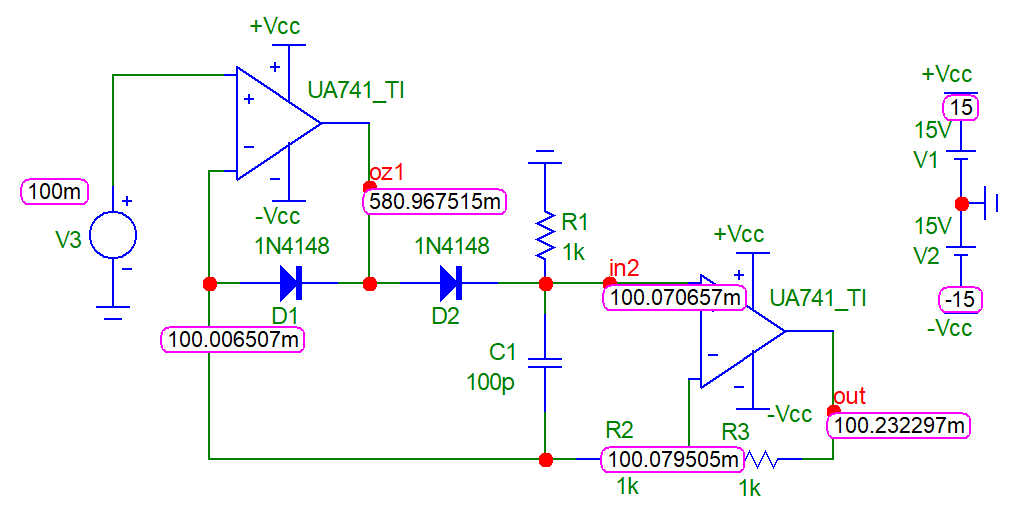
\includegraphics[width=0.8\textwidth]{microcap/3-dcbod.png}
    \caption{Zapojení c) -- stejnosměrný prac. bod při kladném napětí na vstupu, na výstupu kladné napětí.}
    \label{fig:microcap/.png}
\end{figure}

\begin{figure}[h!]
    \centering
    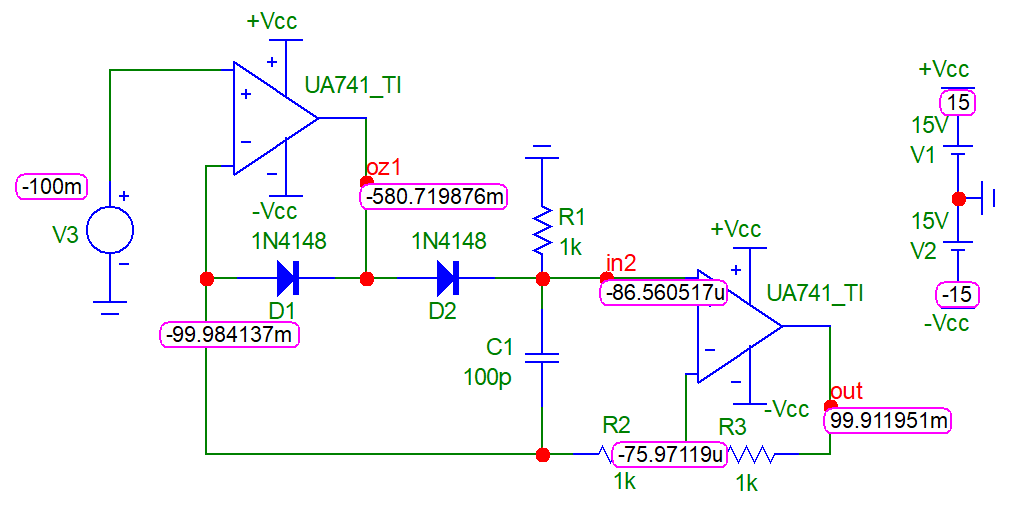
\includegraphics[width=0.8\textwidth]{microcap/3-dcbod2.png}
    \caption{Zapojení c) -- stejnosměrný prac. bod při záporném napětí na vstupu, na výstupu kladné napětí.}
    \label{fig:microcap/.png}
\end{figure}

\begin{figure}[h!]
    \centering
    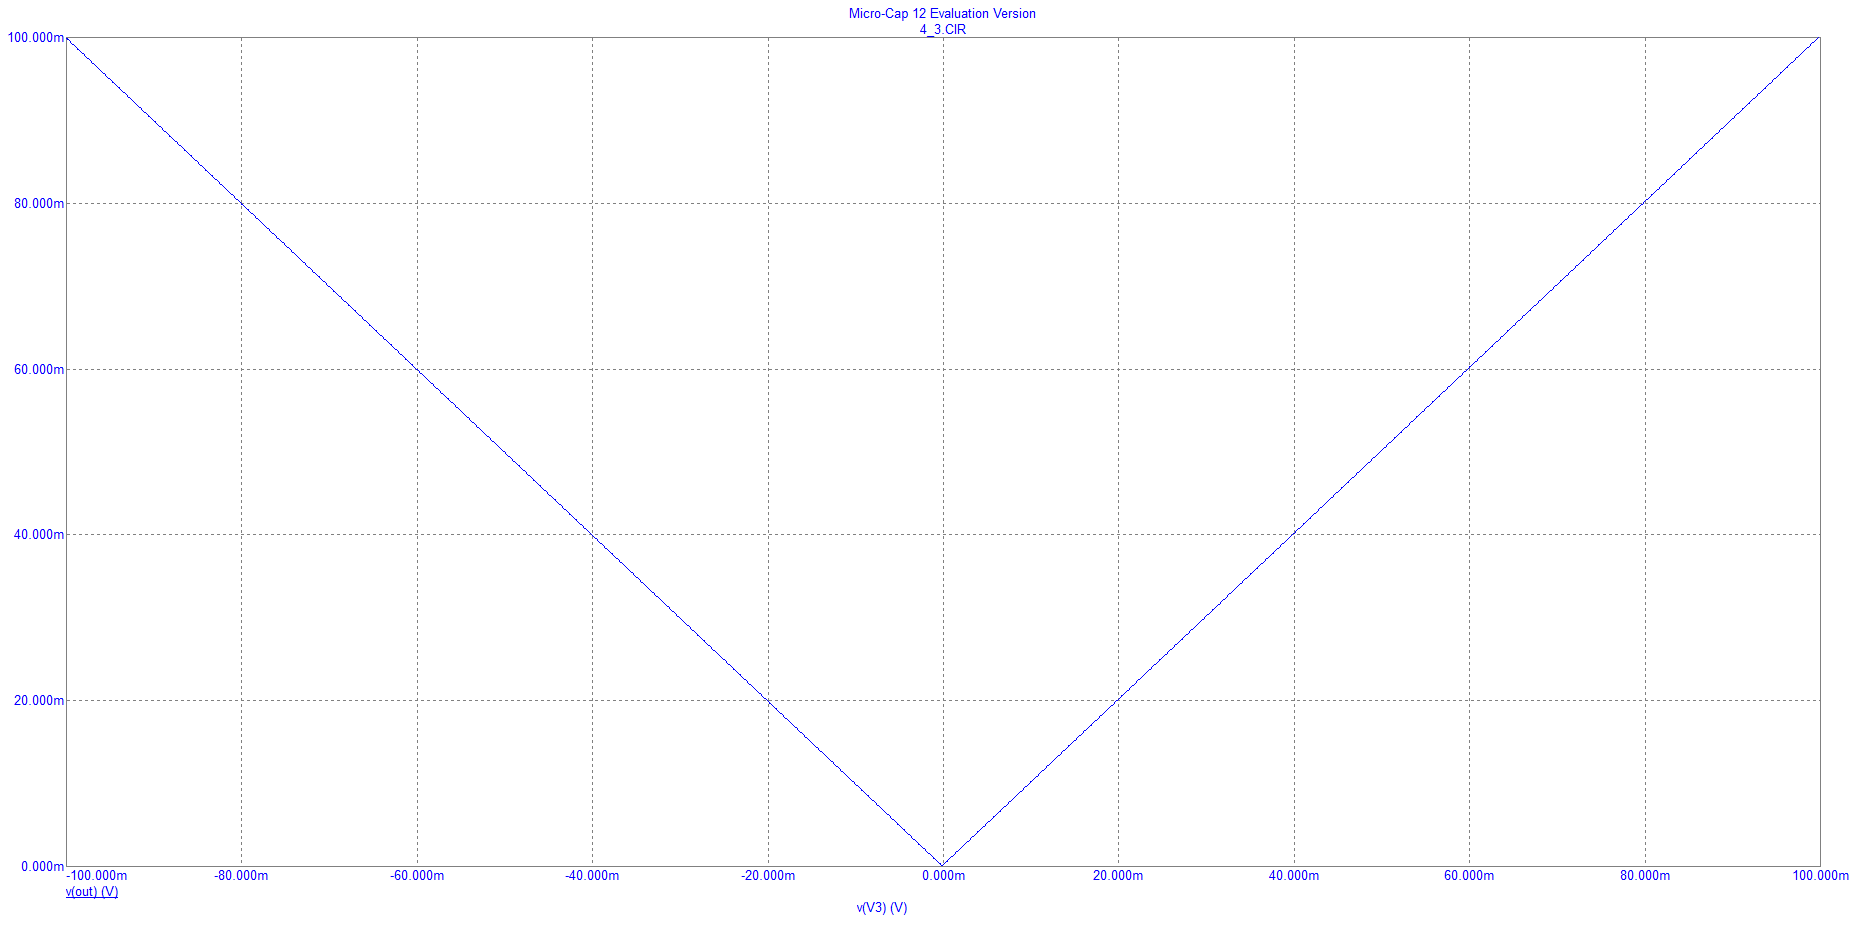
\includegraphics[width=0.8\textwidth]{microcap/3-dcprevodni.png}
    \caption{Zapojení c) -- stejnosměrná převodní charakteristika.}
    \label{fig:microcap/.png}
\end{figure}

\begin{figure}[h!]
    \centering
    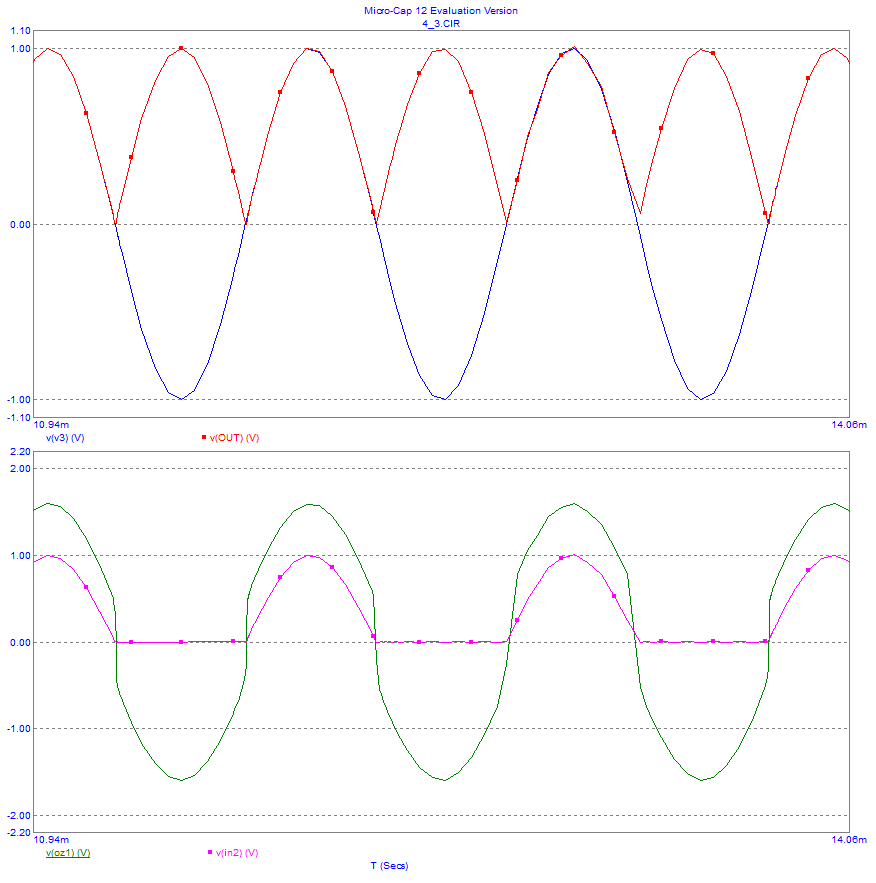
\includegraphics[width=0.66\textwidth]{microcap/3-transient-1khz-1v.png}
    \caption{Zapojení c) -- časová závislost napětí na výstupech obou OZ na vstupním napětí, jednocestné a dvoucestné usměrnění, \(f=\qty{1}{\kilo\hertz}, U_M=\qty{1}{\volt}\).}
    \label{fig:microcap/.png}
\end{figure}

\begin{figure}[h!]
    \centering
    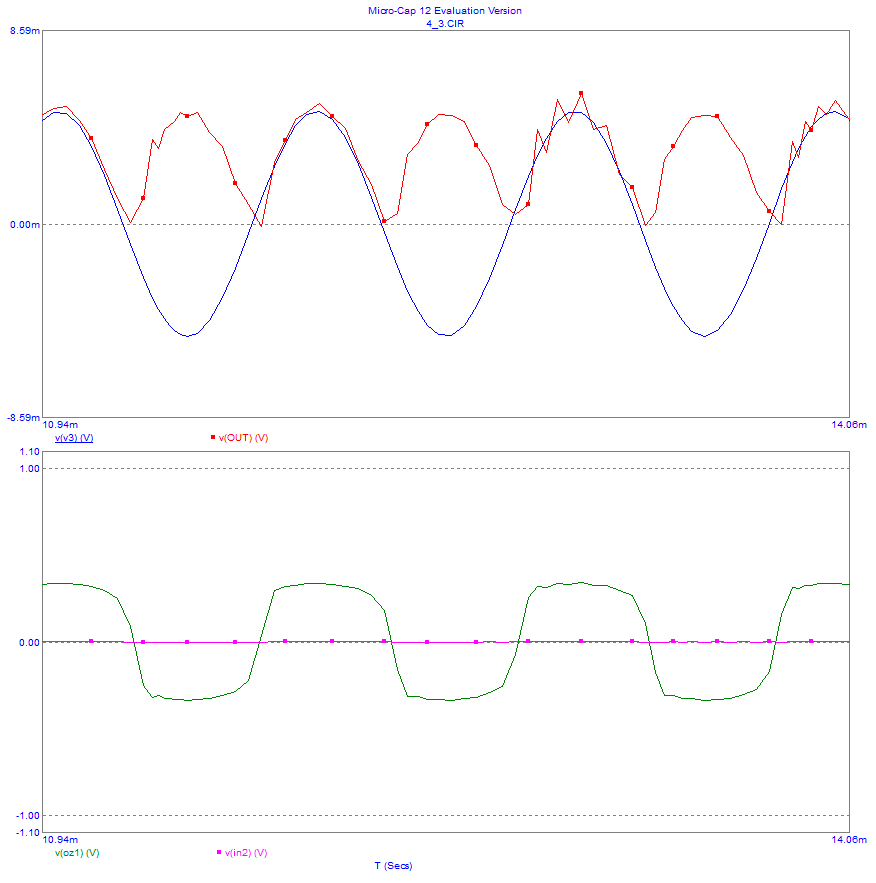
\includegraphics[width=0.66\textwidth]{microcap/3-transient-1khz-5mv.png}
    \caption{Zapojení c) -- časová závislost napětí na výstupech obou OZ na vstupním napětí, nejnižší amplituda, při které uspokojivě usměrňuje, \(f=\qty{1}{\kilo\hertz}, U_M=\qty{5}{\milli\volt}\).}
    \label{fig:microcap/.png}
\end{figure}

% \begin{figure}[h!]
%     \centering
%     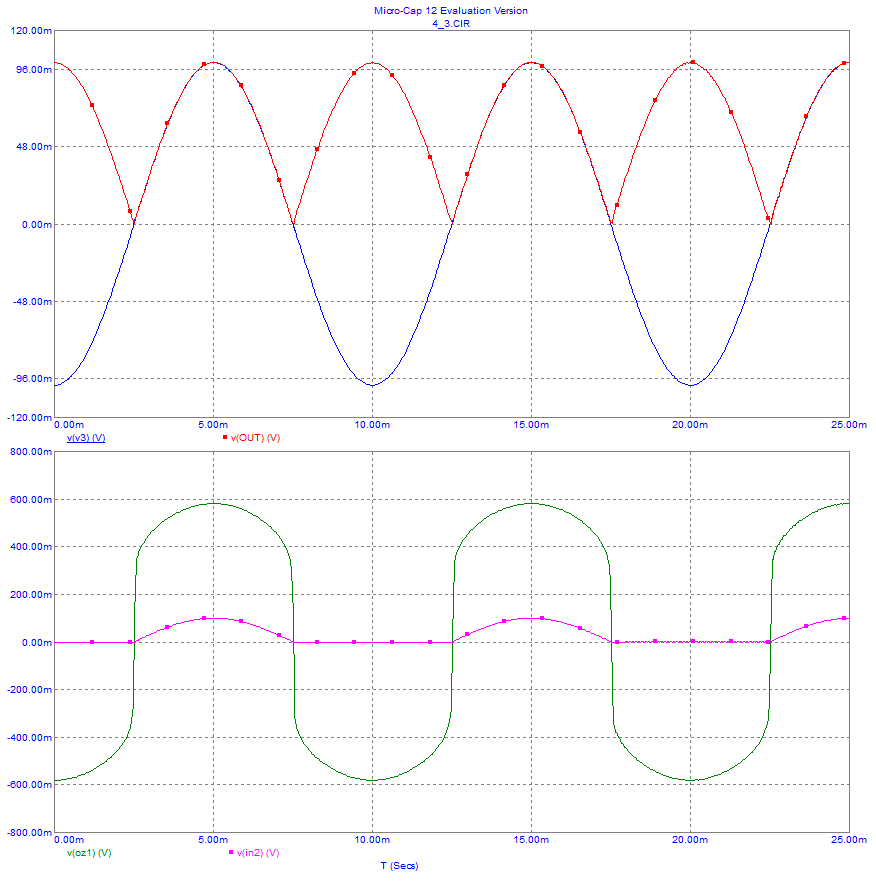
\includegraphics[width=0.8\textwidth]{microcap/3-transient-100hz-0.1v.png}
%     \caption{microcap/.png}
%     \label{fig:microcap/.png}
% \end{figure}

\begin{figure}[h!]
    \centering
    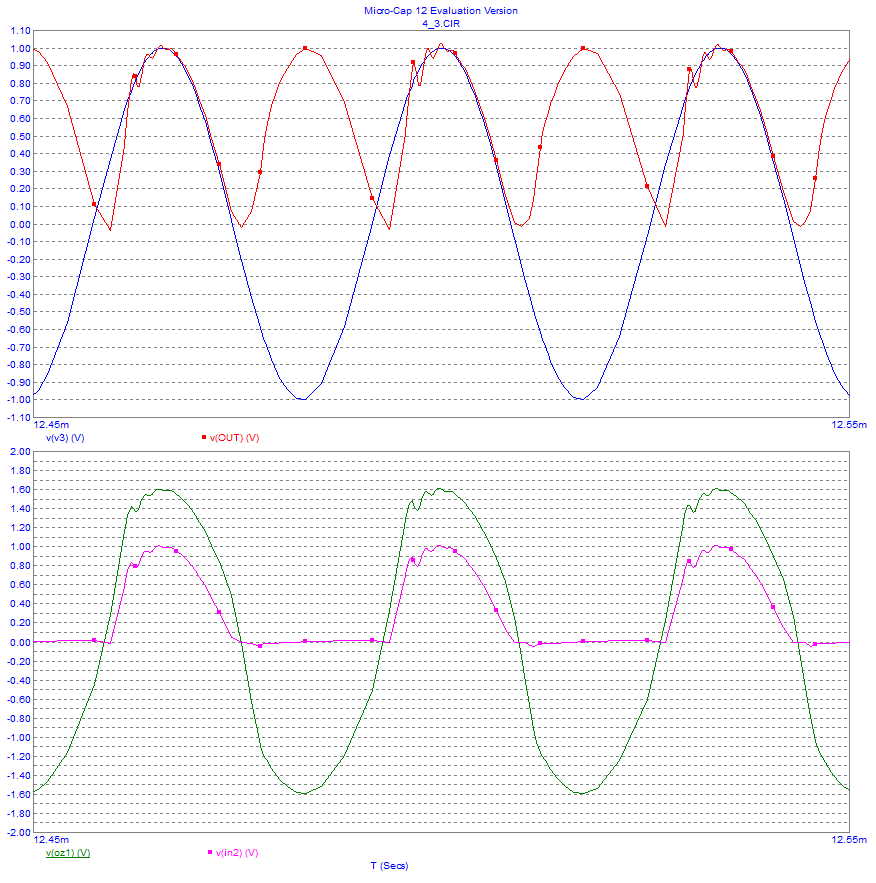
\includegraphics[width=0.8\textwidth]{microcap/3-transient-30khz-1v.png}
    \caption{Zapojení c) -- časová závislost napětí na výstupech obou OZ na vstupním napětí, nejvyšší frekvence, při které uspokojivě usměrňuje, \(f=\qty{30}{\kilo\hertz}, U_M=\qty{1}{\volt}\).}
    \label{fig:microcap/.png}
\end{figure}


%		
%	\clearpage

\section{1. - 4.}
\begin{table}[h!]
	\centering
	\def\arraystretch{1.4}
	\begin{tabular}{ |l|l|l|l|l|l| }
		\hline
		Popis & $ \Delta T$\ [\unit{\kelvin}] & $ U $\ [\unit{\volt}] & $ I $\ [\unit{\ampere}]& $ P $\ [\unit{\watt}] & $ \alpha $\ [\unit{\volt\per\kelvin}] 
		\DTLforeach{prvni}{\A=popis,\B=deltaT,\C=U,\I=I,\D=P,\E=alpha}
		{\DTLiffirstrow{\\ \hline \hline}{\\ \hline} %
			\A & \num[round-mode=places,round-precision=2]{\B} & \num[round-mode=places,round-precision=2]{\C} &
			\num[round-mode=places,round-precision=3]{\I} & 
			\num[round-mode=places,round-precision=3]{\D} & \num[round-mode=places,round-precision=4]{\E}}\\ \hline
	\end{tabular}
	\caption{\label{tab:tabulka-vykon} Tabulka naměřených a vypočtených hodnot.}
\end{table}

\begin{figure*}[h!]
	\begin{tikzpicture}
		\centering
		\begin{axis}
			[
			ylabel={$U\ [\unit{\volt}]$},
			xlabel={$\Delta T\ [\unit{\kelvin}]$},
			axis y line*=left,
			width=1\textwidth,
			height = 0.5\textwidth,
			legend pos=north west,
%			xmin=0,
%			ymin=0,
			xmax=125
			]
			\addplot[mark=x, thick, blue, only marks, mark size=3pt] table [skip first n=2, x=deltaT, y=U, col sep=comma] {data/u-na-deltaT.csv};
			
			\addlegendentry{U}
			
		\end{axis}   
	 
		\begin{axis}
			[
			ylabel={$P\ [\unit{\milli\watt}]$},
			axis x line=none,
			axis y line*=right,
			width=1\textwidth,
			height = 0.5\textwidth,
			legend pos=north east,
			%			xmin=0,
			%			ymin=0,
						xmax=125
			]
			\addplot[mark=+, thick, red, only marks, mark size=3pt] table [skip first n=2, x=deltaT, y=P, col sep=comma] {data/u-na-deltaT.csv};
			
			\addlegendentry{P}
		
	\end{axis}    
	\end{tikzpicture}
	\caption{Závislost termoelektrického napětí $ U $ a výkonu $ P $ generovaných termočlánkem na rozdílu teplot vodních lázní.}
\end{figure*}

Příklady výpočtu:
$$ P=I\cdot  U= 0,019\cdot 0,14\doteq \SI{2,59}{\watt} $$
$$ \alpha= \frac{U}{\Delta T}= \frac{0,14}{13,5}\doteq \SI{0,0104}{\volt\per\meter} $$




\clearpage
\section{7. - 10.}
\begin{table}[h!]
	\centering
	\def\arraystretch{1.4}
	\begin{tabular}{ |l|l|l|l|l| }
		\hline
		$ \tau $\ [\unit{\second}] & $ T_{C-5V} $\ [\unit{\kelvin}] & $ T_{H-5V} $\ [\unit{\kelvin}]& $ T_{C-10V} $\ [\unit{\kelvin}] & $ T_{H-10V} $\ [\unit{\kelvin}]
		\DTLforeach{casova}{\A=t,\B=TC5V,\C=TH5V,\D=TC10V,\E=TH10V}
		{\DTLiffirstrow{\\ \hline \hline}{\\ \hline} %
			\A & \B & \C & \D & \E}\\ \hline
%		
%					\A & \num[round-mode=places,round-precision=2]{\B} & \num[round-mode=places,round-precision=2]{\C} &
%		\num[round-mode=places,round-precision=3]{\D} & \num[round-mode=places,round-precision=4]{\E}}\\ \hline
	\end{tabular}
	\caption{\label{tab:tabulka-vykon} Tabulka naměřených teplot.}
\end{table}

 Z následujících vztahů vypočteme energii potřebnou pro ohřev a ochlazení jednotlivých kapalin a chladící / ohřevný výkon článku v dané situaci. Z našeho měření víme, že hmotnost vody v nádobě je zhruba \SI{175}{\gram}.
	$$ Q=m\cdot c_v(T_2-T_1) $$
	$$ P=\frac{Q}{\tau} $$
		5V ohřev:
	$$ Q_1=0,175\cdot 4180(22,4-20,2)=\SI{1609,3}{\joule} $$
	$$ P_1= \frac{1609,3}{330}\doteq \SI{4,88}{\watt} $$
		5V chlazení:
	$$ Q_2=0,175\cdot 4180(19,7-20,2)=\SI{-365,75}{\joule} $$
	$$ P_2= \frac{-365,75}{330}\doteq \SI{-1,11}{\watt} $$
		10V ohřev:
	$$ Q_3=0,175\cdot 4180(23,2-19,9)=\SI{2413,95}{\joule} $$
	$$ P_3= \frac{2413,95}{300}\doteq \SI{8,05}{\watt} $$
		10V chlazení:
	$$ Q_4=0,175\cdot 4180(18,9-19,9)=\SI{-731,5}{\joule} $$
	$$ P_4= \frac{-731,5}{300}\doteq \SI{-2,44}{\watt} $$
	
	
	\begin{figure*}[h!]
		\begin{tikzpicture}
			\centering
			\begin{axis}
				[
				ylabel={$T\ [\unit{\degreeCelsius}]$},
				xlabel={$t\ [\unit{\second}]$},
				width=1\textwidth,
				height = 0.48\textwidth,
				legend pos=north west,
				%			xmin=0,
				%			ymin=0,
				%			xmax=12.5
				]
				\addplot[mark=triangle, thick, blue, only marks, mark size=3pt] table [skip first n=0, x=t, y=TC5V, col sep=comma] {data/casova-zavislost.csv};
				\addlegendentry{5V, teplota stud. lázně }
				\addplot[mark=triangle*, thick, red, only marks, mark size=3pt] table [skip first n=0, x=t, y=TH5V, col sep=comma] {data/casova-zavislost.csv};
				\addlegendentry{5V, teplota hor. lázně}
				%			\addplot[mark=x, thick, blue, only marks, mark size=3pt] table [skip first n=0, x=t, y=deltaT5V, col sep=comma] {data/casova-zavislost.csv};
				
				\addplot[mark=Mercedes star flipped, thick, blue, only marks, mark size=3pt] table [skip first n=0, x=t, y=TC10V, col sep=comma] {data/casova-zavislost.csv};
				\addlegendentry{10V, teplota stud. lázně}
				\addplot[mark=Mercedes star, thick, red, only marks, mark size=3pt] table [skip first n=0, x=t, y=TH10V, col sep=comma] {data/casova-zavislost.csv};
				\addlegendentry{10V, teplota hor. lázně}
				%			\addplot[mark=x, thick, blue, only marks, mark size=3pt] table [skip first n=0, x=t, y=deltaT10V, col sep=comma] {data/casova-zavislost.csv};
				
				%			\addlegendentry{Naměřené hodnoty}
				
			\end{axis}    
		\end{tikzpicture}
		\caption{Časová závislost teplot lázní ohřívaných (resp. chlazených) připojením napětí zdroje k termočlánku.}
	\end{figure*}
	
	\begin{figure*}[h!]
		\begin{tikzpicture}
			\centering
			\begin{axis}
				[
				ylabel={$\Delta T\ [\unit{\kelvin}]$},
				xlabel={$t\ [\unit{\second}]$},
				width=1\textwidth,
				height = 0.48\textwidth,
				legend pos=north west,
				%			xmin=0,
				%			ymin=0,
				%			xmax=12.5
				]
				
				
				\addplot[mark=triangle, thick, blue, only marks, mark size=3pt] table [skip first n=0, x=t, y=deltaT5V, col sep=comma] {data/casova-zavislost.csv};
				\addlegendentry{5V, rozdíl teplot lázní}
				
				\addplot[mark=Mercedes star, thick, red, only marks, mark size=3pt] table [skip first n=0, x=t, y=deltaT10V, col sep=comma] {data/casova-zavislost.csv};
				\addlegendentry{10V, rozdíl teplot lázní}
				
				
			\end{axis}    
		\end{tikzpicture}
		\caption{Časová závislost rozdílů teplot lázní $ \Delta T $ vytvořeného připojením napětí zdroje k termočlánku.}
	\end{figure*}
	
	

		
	% \clearpage
\section{Závěr}
	Měřili jsme peltierův článek zapojený jak ve funkci zdroje napětí, tak ve funkci chladiče / ohřívače. Pokud k plošky článku přiložíme k materiálům s různou teplotou, na výstupu článku vznikne elektrické napětí úměrné rozdílu teplot. Z počtu bodů, které jsme měřili, nelze přesný charakter závislosti spolehlivě určit, dle dostupné teorie by měl ale odpovídat přímce. Také jsme se pokusili stanovit Seebeckův koeficient našeho článku, který nám vyšel v rozmezí 0,003 až 0,01 \unit{\volt\per\kelvin}.
	
	Při druhém zapojení jsme nechali článkem protékat proud a měřili jsme změnu teploty vody v nádobkách. Vzniklý teplotní rozdíl je závislý na připojením napětí, větší napští odpovídá většímu chladícímu i ohřevnému výkonu, článek tak zvládá déle "vzdorovat" tepelné výměně s okolním prostředím.

\end{document}